\hypertarget{group__Harasser}{\section{Harasser}
\label{group__Harasser}\index{Harasser@{Harasser}}
}


\hyperlink{namespaceHarasser}{Harasser} tools for test content.  


Collaboration diagram for Harasser\-:
\nopagebreak
\begin{figure}[H]
\begin{center}
\leavevmode
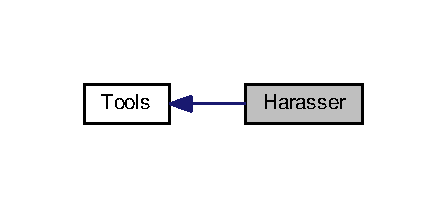
\includegraphics[width=214pt]{group__Harasser}
\end{center}
\end{figure}
\hyperlink{namespaceHarasser}{Harasser} tools for test content. \hypertarget{group__Harasser_Harasser}{}\subsection{Harasser}\label{group__Harasser_Harasser}
Run harasser scripts while test-\/content is running 
\begin{DoxyParams}{Parameters}
{\em trigger\-\_\-scripts} & Scripts to run to launch harassers \\
\hline
{\em stop\-\_\-scripts} & Scripts to run to stop and clean-\/up harassers \\
\hline
{\em join\-\_\-timeout} & Seconds to wait for process to finish \\
\hline
\end{DoxyParams}
